% MX17 thermal-window (>1 ms) SiPM/plastic trigger optimization
% Build:  pdflatex thermal_trigger.tex  (run twice for the outline/refs)
\documentclass[aspectratio=169,10pt]{beamer}
\usetheme{default}
\usecolortheme{seahorse}
\usepackage{graphicx}
\usepackage{booktabs}
\usepackage{colortbl}
\usepackage{amsmath}
\usepackage{tikz}
\usetikzlibrary{arrows.meta,positioning}

\graphicspath{{figs/}}
\setbeamertemplate{navigation symbols}{}
\setbeamertemplate{footline}[frame number]
\definecolor{mxnavy}{RGB}{31,58,95}
\definecolor{mxred}{RGB}{200,40,40}
\definecolor{mxgreen}{RGB}{40,140,60}
\setbeamercolor{frametitle}{fg=mxnavy}
\setbeamercolor{structure}{fg=mxnavy}
\newcommand{\keybox}[1]{\begin{beamercolorbox}[wd=\textwidth,sep=4pt,rounded=true]{block body}%
  \color{mxnavy}\small #1\end{beamercolorbox}}
\newcommand{\unit}[1]{\,\mathrm{#1}}

\title[MX17 thermal trigger]{MX17 --- Thermal-window ($>1$\,ms) Trigger Optimization}
\subtitle{SiPM wall $\times$ plastics: tagging X17 \& IPC pairs, rejecting capture-$\gamma$ background}
\author{Geant4 full-simulation study}
\date{2026-07-19 \quad\textit{(final surveyed geometry)}}

\begin{document}

\begin{frame}[plain]\titlepage\end{frame}

% ---------------------------------------------------------------------------
\begin{frame}{The question}
\textbf{Goal:} with the final geometry, decide how to trigger in the
\emph{thermal neutron} time window (arrival $>1$\,ms after the $\gamma$ flash)
to efficiently tag possible \textbf{X17} and \textbf{IPC} $e^+e^-$ pairs while
rejecting neutron-capture backgrounds.
\vfill
\begin{columns}[T]
\column{0.5\textwidth}
\textbf{Two trigger detectors per arm}
\begin{itemize}
\item \textcolor{mxnavy}{SiPM wall} --- 16 thin (3\,mm) scint bars; gives the
      2-arm pair \emph{topology}.
\item \textcolor{mxnavy}{Plastics} --- 2 thick (2.5\,cm) bars; give
      \emph{energy} (per-leg pulse height).
\end{itemize}
\column{0.5\textwidth}
\textbf{Design levers}
\begin{itemize}
\item SiPM per-bar threshold $a$
\item Plastic per-bar threshold $b$
\item Coincidence topology (1 leg / 2 legs / \dots)
\end{itemize}
\end{columns}
\vfill
\keybox{Both thresholds are quoted in \textbf{MIP} units, so they transfer
directly to hardware via the measured MIP peaks. \;
$1\unit{MIP}=458\unit{keV}$ (SiPM bar), $4.33\unit{MeV}$ (plastic).}
\end{frame}

% ---------------------------------------------------------------------------
\begin{frame}{Setup --- 4-arm detector, top-down}
\begin{columns}[c]
\column{0.62\textwidth}
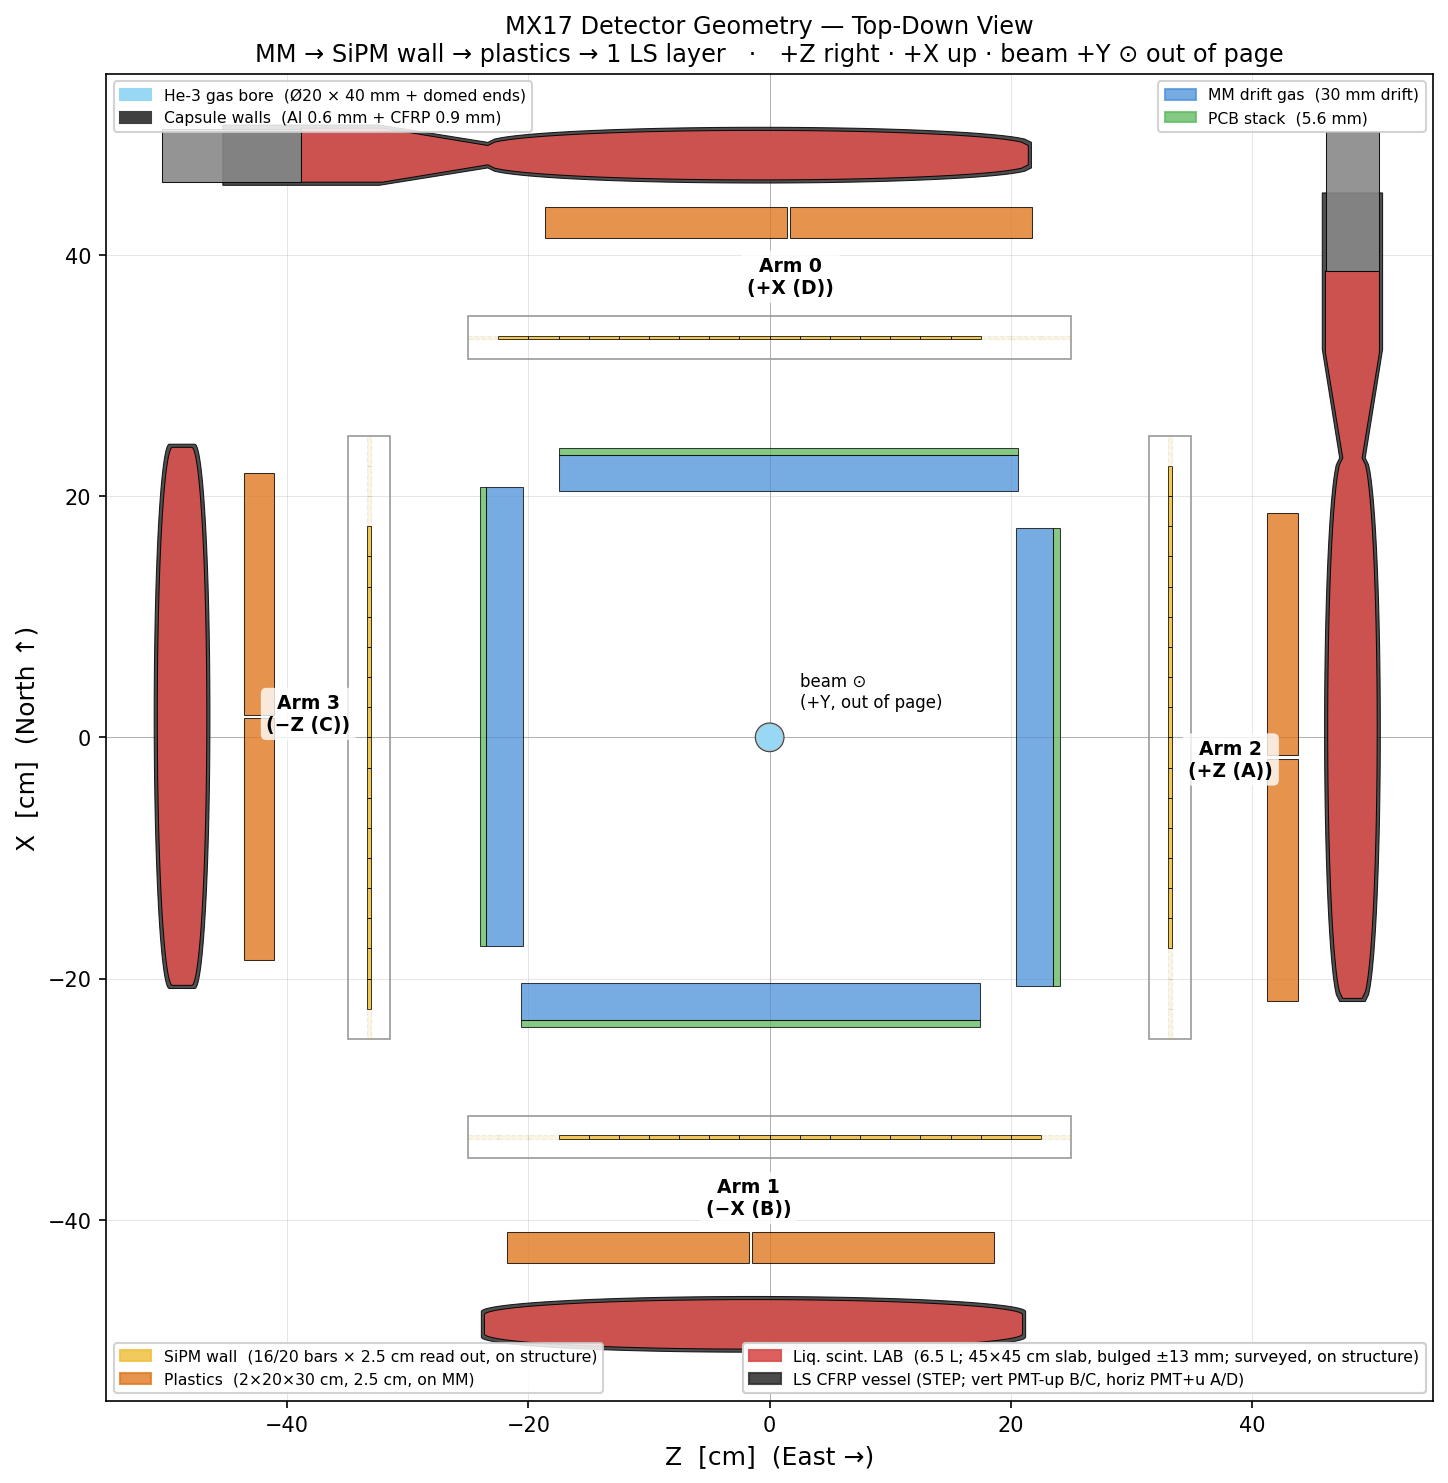
\includegraphics[width=\textwidth]{mx17_geometry_topdown.png}
\column{0.38\textwidth}\small
Beam ($+Y$) into the page; four arms in the transverse plane.\\[4pt]
Stack, inside\,$\to$\,out per arm:
\begin{enumerate}
\item Micromegas (tracking)
\item \textbf{SiPM wall} (trigger)
\item \textbf{plastics} (trigger)
\item liquid-scint layer
\end{enumerate}
\vspace{4pt}
He-3 target at the centre: $\varnothing20\times40$\,mm gas bore in an
Al+CFRP capsule.
\end{columns}
\end{frame}

% ---------------------------------------------------------------------------
\begin{frame}{Setup --- the trigger stack}
\begin{columns}[c]
\column{0.55\textwidth}
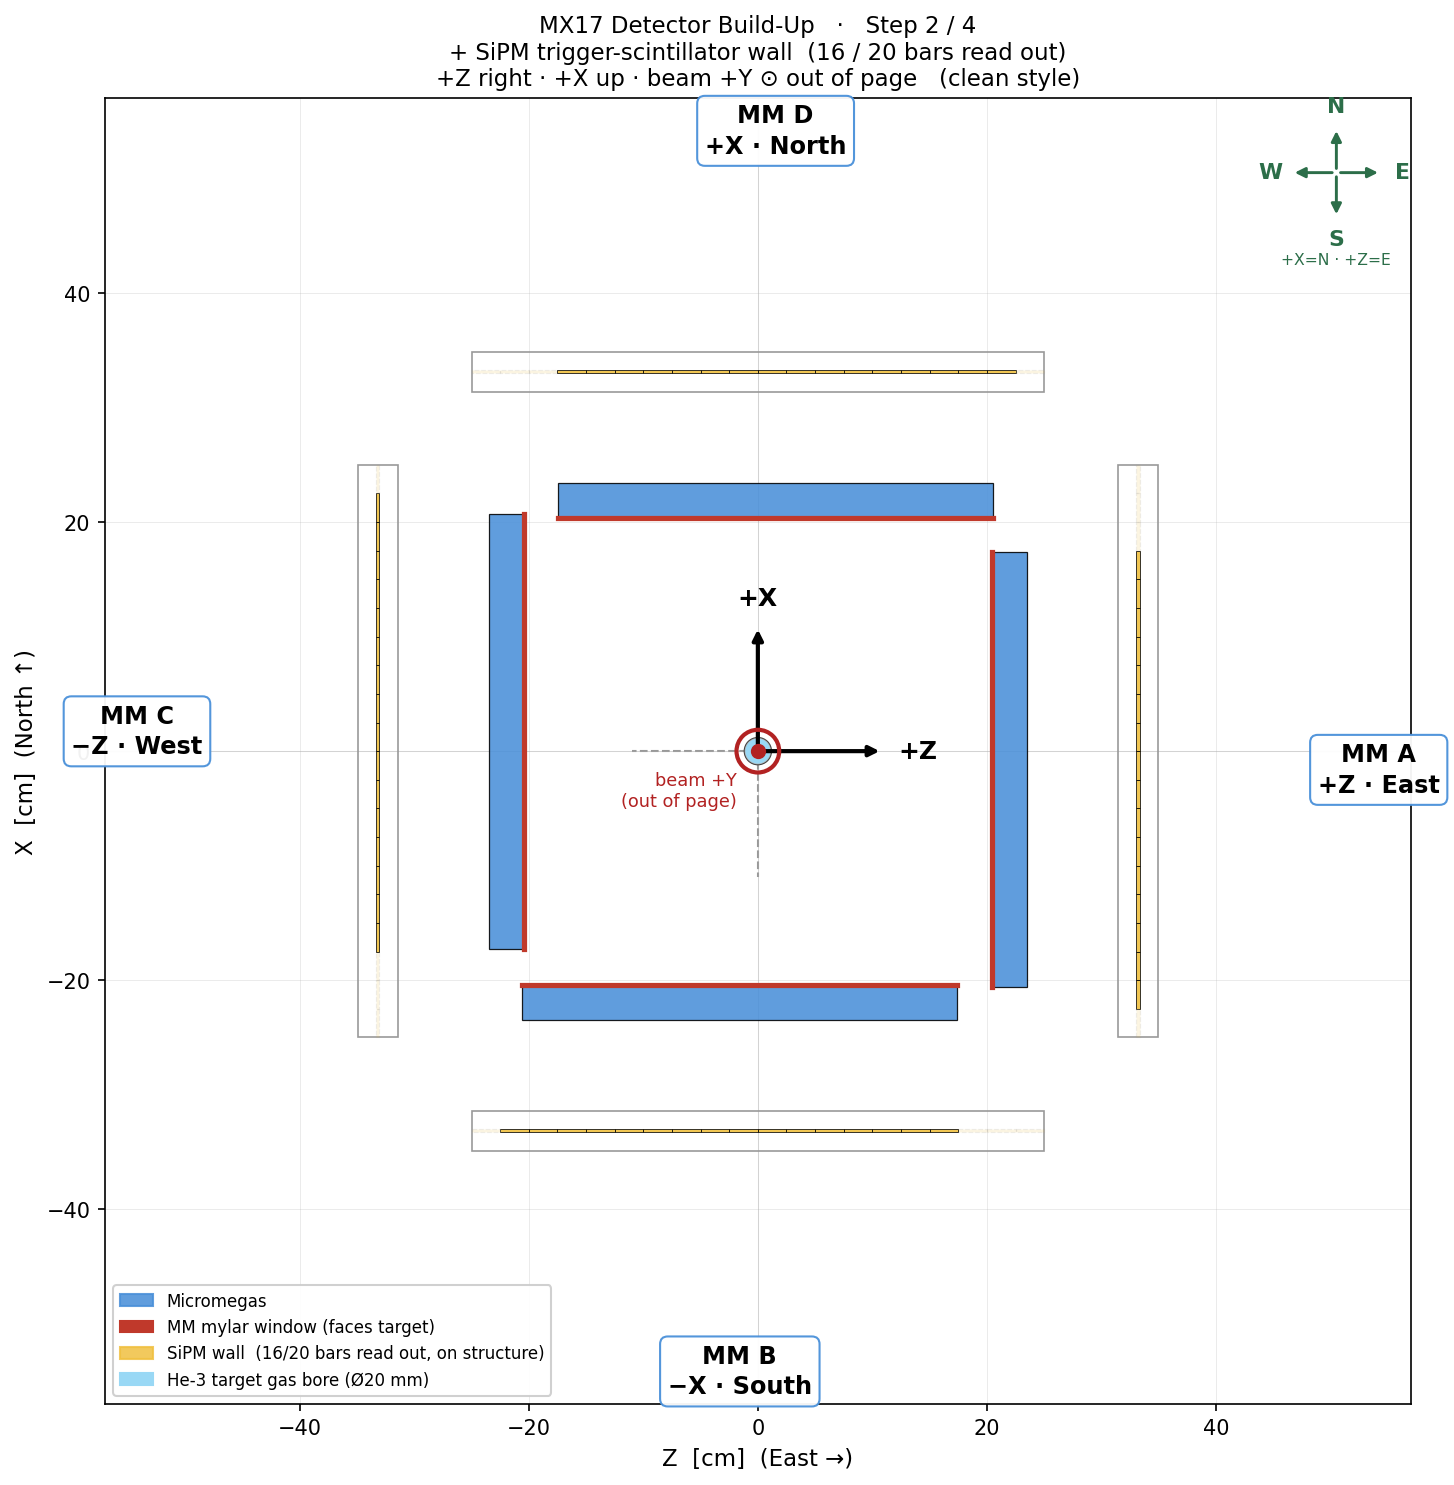
\includegraphics[width=\textwidth]{mx17_buildup_clean_2_sipm.png}
\column{0.45\textwidth}\small
\textbf{SiPM wall} (yellow): 50\,cm span, 16 of 20 bars read out, bars run
along the beam, array along the tangent. Centered on the mechanical structure.\\[6pt]
\textbf{Plastics} (orange): two $20\times30\times2.5$\,cm bars, tape+Al
wrapped, behind the wall, centered on the Micromegas.\\[6pt]
A leg ``fires'' when its SiPM bar \emph{and} a plastic bar are both above
threshold.
\end{columns}
\end{frame}

% ---------------------------------------------------------------------------
\begin{frame}{Simulation}
\begin{columns}[T]
\column{0.54\textwidth}
\textbf{Campaigns} (Geant4 11.2, FTFP\_BERT\_HP; final geometry;
all files validated):
\smallskip
\begin{tabular}{@{}lll@{}}
\toprule
Run & primaries & purpose\\
\midrule
thermal $n$ & $10^{9}$ & in-gate bkg\\
            & 1\,meV--2\,eV & \\
epi $n$     & $5\times10^{8}$ & spill-in\\
            & 2\,eV--100\,keV & check\\
pairs       & $10^{7}$ & X17+IPC\\
            & 50/50 & signal\\
\bottomrule
\end{tabular}
\column{0.46\textwidth}
\textbf{Two physics details that matter}
\begin{itemize}\small
\item \textbf{Self-shielding:} thermal captures sit within $\sim$mm of the gas
      entrance (median 14\,mm depth, 95\% $<25$\,mm). Pair vertices are sampled
      from the \emph{measured} capture profile, not uniform-in-gas
      ($\sim$3.7\,cm upstream of centre).
\item \textbf{Gate $\leftrightarrow$ energy:}
      $\mathrm{TOF}[\mathrm{ms}]=1.41/\sqrt{E_n[\mathrm{eV}]}$ at 19.5\,m;
      $>1$\,ms $\Leftrightarrow E_n<2$\,eV, $4.28\times10^{6}\,n$/pulse.
\end{itemize}
\end{columns}
\vfill
\keybox{Geant4 has no internal pair conversion --- X17 and IPC are explicit
generator modes; the neutron runs supply the capture-$\gamma$ background and
all singles.}
\end{frame}

% ---------------------------------------------------------------------------
\begin{frame}{Trigger observables --- per-arm pulse height in MIP units}
\begin{columns}[c]
\column{0.6\textwidth}
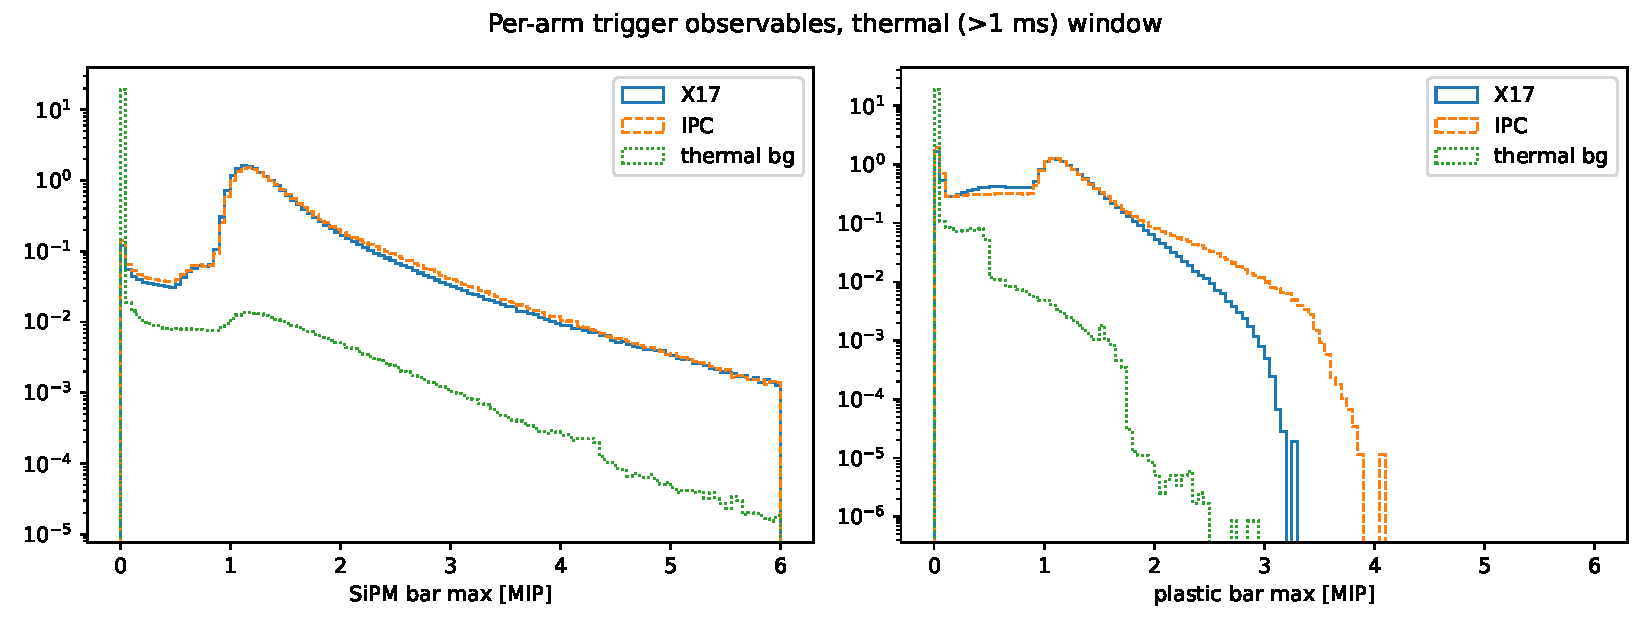
\includegraphics[width=\textwidth]{trigger_spectra.pdf}
\column{0.4\textwidth}\small
\textbf{Signal legs} peak at 1\,MIP (crossing $e^\pm$); stopped legs reach
$\sim$3\,MIP in the plastic.\\[6pt]
\textbf{Background} (thermal captures):
\begin{itemize}
\item plastic hits die above $\sim$1.7\,MIP --- the $^{28}$Al 7.72\,MeV
      Compton edge; H-capture 2.22\,MeV $\gamma$ stays $<0.5$\,MIP.
\item SiPM shows no MIP peak ($\gamma$ Comptons only).
\end{itemize}
\smallskip
$\Rightarrow$ the \textbf{plastic} pulse height is the background-rejection
lever.
\end{columns}
\end{frame}

% ---------------------------------------------------------------------------
\begin{frame}{Topology: full coincidence costs efficiency, but is clean}
\centering
\begin{tabular}{@{}lccc@{}}
\toprule
Pair trigger (both arms) & $\varepsilon$(X17) & $\varepsilon$(IPC) & bkg pair-tags/pulse\\
\midrule
SiPM-only (2 arms $\geq0.5$) & 15.0\% & --- & 42 \\
2 SiPM + $\geq1$ plastic confirm & 7.0\% & 5.3\% & 1.8 \\
\textbf{full: 2$\times$(SiPM$\times$plastic)} & \textbf{2.1\%} & \textbf{0.7\%} & \textbf{0.17} \\
\bottomrule
\end{tabular}
\vfill
\begin{itemize}
\item Requiring the plastic on \emph{both} legs costs $\sim5\times$ in signal
      --- pure solid angle (plastics are smaller and further back).
\item \textbf{This study assumes the full coincidence} (the clean, high-purity
      choice), and optimizes the plastic threshold $b$ within it.
\end{itemize}
\end{frame}

% ---------------------------------------------------------------------------
\begin{frame}{Key result: the plastic threshold does \emph{not} reject IPC}
\begin{columns}[c]
\column{0.62\textwidth}
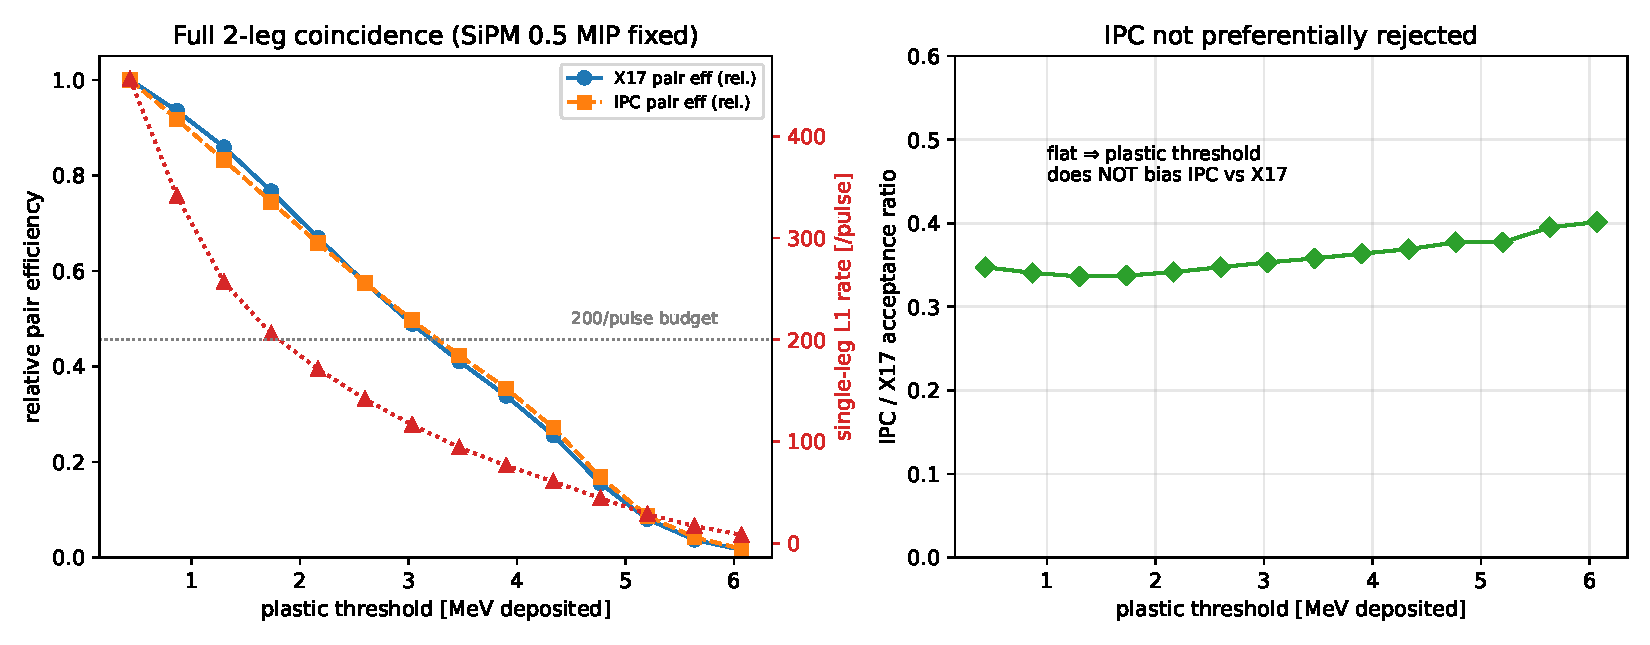
\includegraphics[width=\textwidth]{ipc_plastic_threshold.pdf}
\column{0.38\textwidth}\small
IPC/X17 acceptance ratio is \textbf{flat} ($\sim$0.35) across the whole
threshold range.\\[6pt]
\textbf{Why:} IPC's $1/M_{ee}$ spectrum favours soft, collinear pairs ---
97\% of triggering IPC has both legs in the \emph{same} arm and is lost to the
2-arm requirement \emph{on geometry}, before any energy cut.\\[6pt]
The surviving IPC looks kinematically like X17, so $b$ cuts them in lockstep.
\end{columns}
\vfill
\keybox{You may raise the plastic threshold freely for background/rate control:
it costs total statistics, \textbf{not} the IPC-vs-X17 balance.}
\end{frame}

% ---------------------------------------------------------------------------
\begin{frame}{Signal-to-noise optimization}
\begin{columns}[c]
\column{0.63\textwidth}
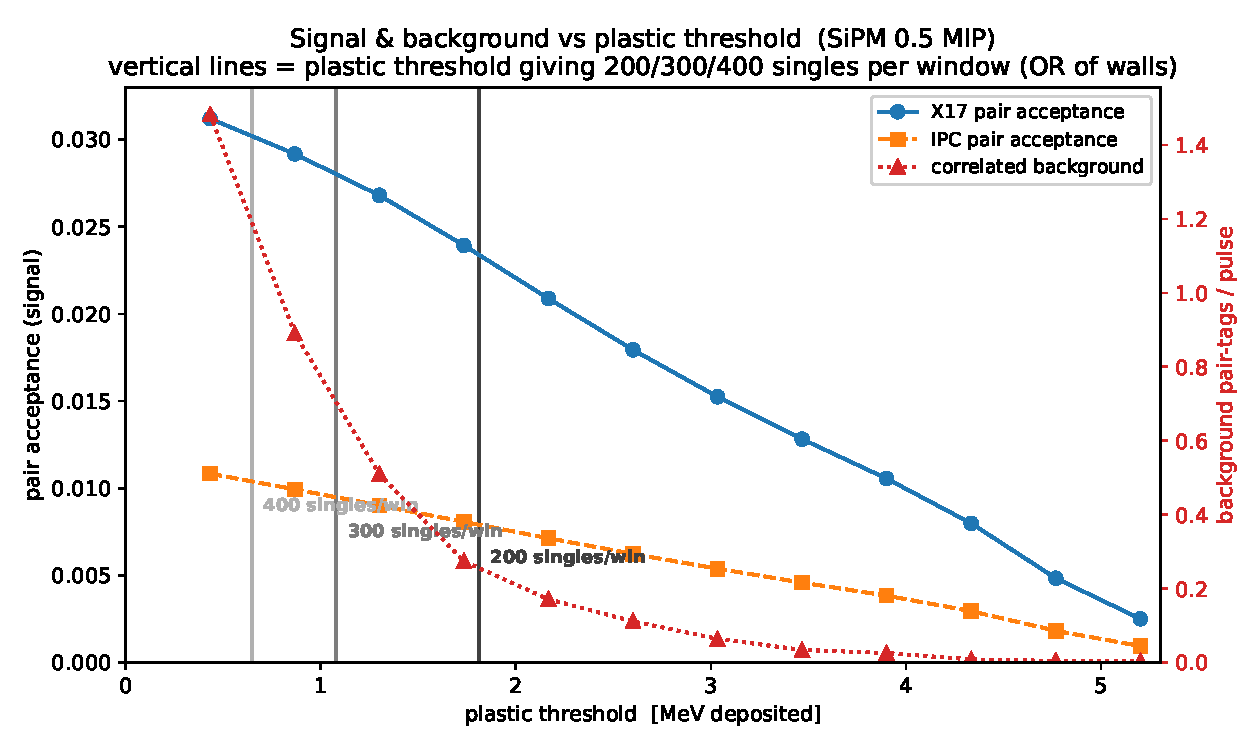
\includegraphics[width=\textwidth]{threshold_linear.pdf}
\column{0.37\textwidth}\small
Signal (left, blue/orange) falls \emph{gently}; the correlated capture
background (right, red) \textbf{collapses by $\sim$1.5\,MeV} once you clear the
capture-$\gamma$ Compton edges.\\[5pt]
So S/N keeps improving with threshold --- the cost is total statistics, not
the IPC/X17 balance.\\[5pt]
Vertical lines: the plastic threshold at which the (simulated) singles rate ---
the \textbf{OR of all four walls} --- equals 200 / 300 / 400 per window, i.e.\
the DAQ capacity ceilings.
\end{columns}
\vfill
\keybox{Sweet spot \textbf{plastic $\approx$ 2--3\,MeV}: background already
$<0.1$/pulse, $\sim$50--65\% of X17 \& IPC kept, IPC/X17 undistorted, and the
singles rate is under the 200/window DAQ ceiling.}
\end{frame}

% ---------------------------------------------------------------------------
\begin{frame}{Rate budget \& the S/N table}
\centering
\small
\begin{tabular}{@{}rccccc@{}}
\toprule
plastic & $\varepsilon$(X17) & $\varepsilon$(IPC) & corr.\ bkg & single-leg & \\
$[$MeV$]$ & pair & pair & /pulse & rate/pulse & \\
\midrule
0.9 & 0.029 & 0.010 & 0.89 & 341 & \\
1.7 & 0.024 & 0.008 & 0.27 & 206 & $\leftarrow$ 200 budget\\
\rowcolor{green!12}
2.6 & 0.018 & 0.006 & 0.11 & 142 & \textbf{recommended}\\
3.0 & 0.015 & 0.005 & 0.06 & 116 & \\
3.5 & 0.013 & 0.005 & 0.03 & \phantom{0}94 & MC floor\\
\bottomrule
\end{tabular}
\vfill
\begin{itemize}\small
\item \textbf{Measured DAQ capacity} (\texttt{zs\_ipd\_safety}, 2026-07-18):
      $\sim$101 ev/window at IPD=10 (clean), $\sim$189 at IPD=5, $\sim$226 at
      IPD=2 --- so the \textbf{200/window budget is real} (aggressive today;
      300--400 awaits the network upgrade).
\item Single-leg (L1) singles are the DAQ constraint --- the \emph{pair}
      coincidence is $<2$/pulse. If the 2-arm coincidence is formed in
      hardware, $b$ can go as low as you like.
\item \textbf{Singles caveat:} the vertical lines use \emph{simulated} singles
      ($\sim$450--550/window at the floor), $\sim2\times$ below the DAQ-measured
      trigger level --- so the true 200/300/400 thresholds sit somewhat higher.
      Re-anchor once a clean scaler-based singles-vs-threshold scan exists
      (M5 scaler was dead in the July run).
\end{itemize}
\end{frame}

% ---------------------------------------------------------------------------
\begin{frame}{Summary \& recommendation}
\begin{itemize}
\item \textbf{Trigger:} full 2-arm SiPM$\times$plastic coincidence,
      SiPM $\geq0.5$\,MIP, \textbf{plastic $\approx$ 2.6--3.0\,MeV
      (0.6--0.7\,MIP)}.
\item \textbf{Keeps both signals:} the plastic threshold does not bias IPC vs
      X17 (flat ratio); it trades total statistics for purity.
\item \textbf{S/N-optimal in the measurable range}, correlated background
      $<0.1$/pulse, comfortably under the single-leg rate budget.
\end{itemize}
\vfill
\textbf{Caveats / next steps}
\begin{itemize}\small
\item Thermal-gate signal production is tiny (self-shielding ceiling
      $\sim10^{-4}$ IPC/pulse) --- this window is background characterization;
      the physics ROI is the $\mu$s-scale MeV window (rates $\times10^4$):
      re-run the same scan there.
\item Accidental (uncorrelated) coincidences scale as (single-leg rate)$^2$;
      full optimization needs the coincidence window --- Python time-domain layer.
\item If the \emph{IPC invariant-mass spectrum} is a goal, keep $b$ lower and
      correct with efficiency (a high $b$ sculpts the accepted $M_{ee}$ shape).
\end{itemize}
\end{frame}

\end{document}
